
\documentclass{beamer}
\usepackage{float}

\usetheme{default}

\title{Version Control Systems(VCS)}

\author{Kiran Vasudev\inst{1}}

\institute[]
{
  \inst{1}
  Hochschule Bonn-Rhein-Sieg

}

\begin{document}

\begin{frame}
  \titlepage
\end{frame}

\begin{frame}{Outline}
  \tableofcontents
\end{frame}

\begin{frame}{What is it?}
\section{What is it?}
  \begin{itemize}
  \item {
    A method to manage file changes over time. These files are stored in a central location.
  }
  \item {
    A backup when things go wrong.
  }
  \item{A software that helps team members collaborate with minimum disruptions.}
  \end{itemize}
\end{frame}

\begin{frame}{Why should we use it ?}
\section{Why should we use it ?}
  \begin{itemize}
  \item {
    A complete long-term change history of every file.
  }
  \item {   
    Branching and merging
  }
  \item {   
    Ability to trace each change made
  }
  \item {   
	Allows multiple developers to work simultaneously
  }
  \end{itemize}
\begin{figure}
	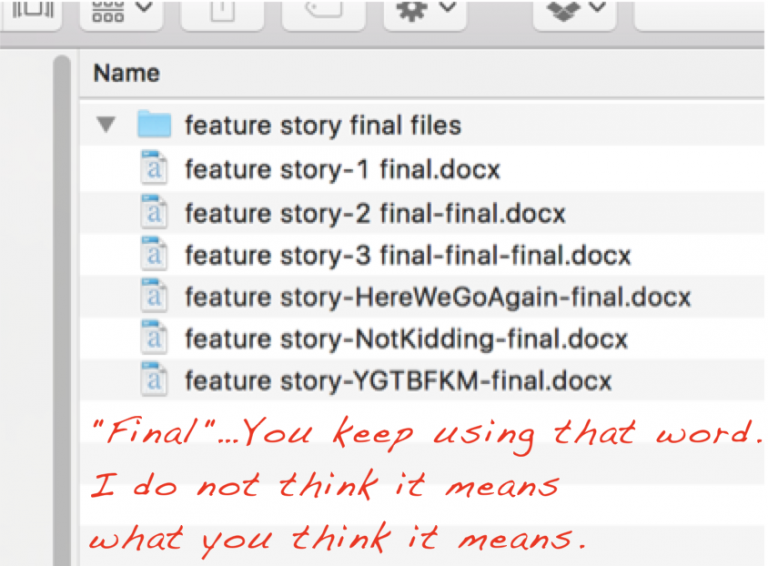
\includegraphics[scale=0.25]{images/final-final}
	\caption{Why we need Version Control\cite{naming-conv}}
\end{figure}
\end{frame}

\begin{frame}{Types of VCS}{Centralized VCS}
\section{Types of VCS}
\subsection{Centralized VCS}
  \begin{columns}
\column{0.5\textwidth}
\begin{itemize}
  \item {
    Centralized VCS keeps the history of changes on a central server.
  }
  \item {
    Designed with the intent that there is only "One True Source"  
  }
  \item {
    If you want to make a copy of your data, you have to copy/paste it, literally.  
  }
  \item{
	Sourceforge.net uses this type of versioning.  
  }
  \item{
      \textbf{Example:} SVN (Subversion)
  }  
  \end{itemize}
\column{0.5\textwidth}
\begin{figure}
	 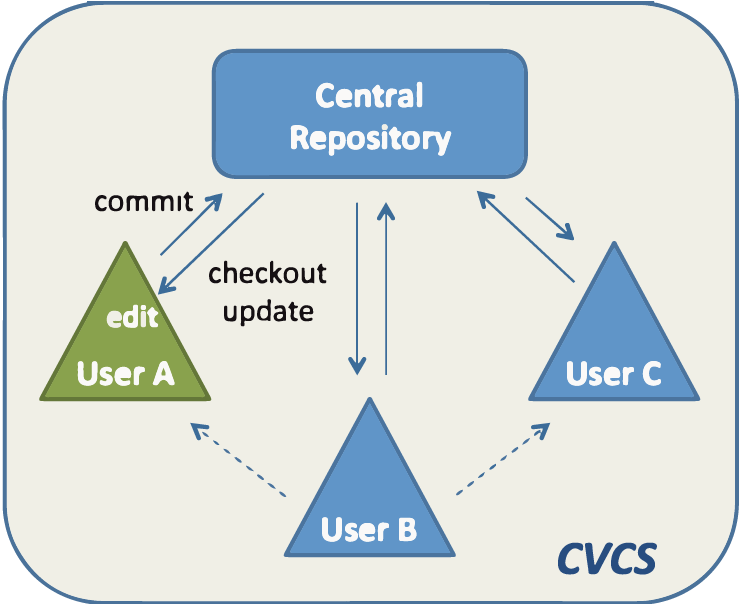
\includegraphics[width=.9\textwidth]{images/cvcs}
	 \caption{Centralized Version System \cite{website}}
 \end{figure}
\end{columns}
\end{frame}	

\begin{frame}{Types of VCS}{Decentralized VCS}
\subsection{Distributed VCS}
\begin{columns}
\column{0.6\textwidth}
\begin{itemize}
		  \item {
		    In distributed VCS, everyone has a local copy of the entire work’s history
		  }
		  \item {
		    Each repository is as good as the other ie. each repository acts as a "True Source".
		  }
		  \item{
			Robust to central server crashes
		  }
		  \item{
			Your local copy is a repository, and you can commit to it and get all benefits of source control - Offline Source Control.
		  }	  
		  \item{
			Mozilla Firefox uses this kind of versioning.  
		  }
		  \item{
           \textbf{ Example: }Almost all open source projects use this type of version control.		  
		  }
	  \end{itemize}
\column{0.4\textwidth}
\begin{figure}
	 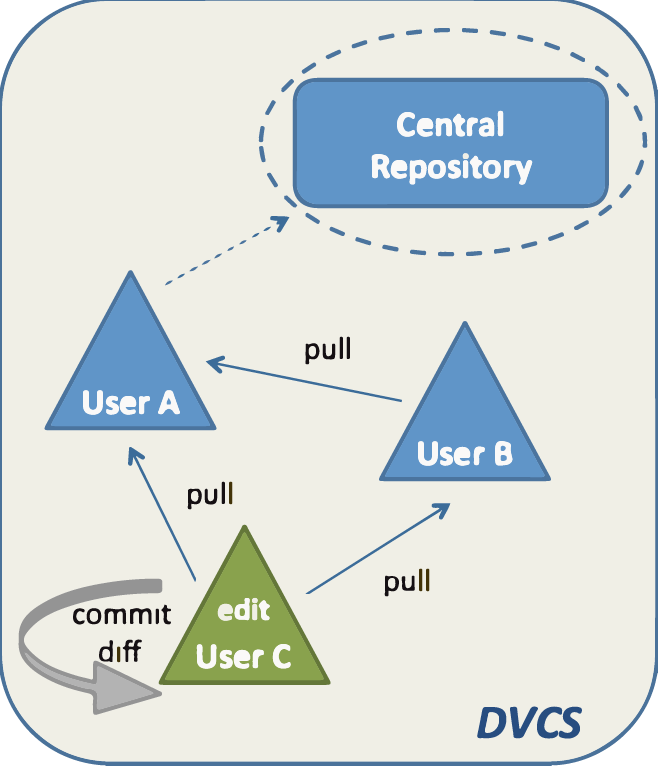
\includegraphics[width=.9\textwidth]{images/dvcs}
	 \caption{Distributed Version System \cite{website}}
 \end{figure}
\end{columns}
\end{frame}	

\begin{frame}[allowframebreaks]{Pros and Cons}{Git vs SVN}
\subsection{Git vs SVN}

\textbf{Pros of using SVN}
\begin{itemize}
    \item Subversion has better GUIs than Git
    \item Working through versions in Git is tougher than SVN. Git uses SHA-1 hashes while SVN uses sequential revision numbers. 
\end{itemize}
\textbf{Pros of using Git}
\begin{itemize}
    \item Git is much faster than SVN as they do not have to keep communicating with a central server when changes are made.
    \item Very secure. Every file and commit is checksummed.
    \item The Git branching model is much better than any other VCS'.
    \item Git repository file formats are simple and hence  repair and corruption is rare. Space requirements are small
    \item As it is a DVCS, scalability is not an issue. 
\end{itemize}
\framebreak
\begin{figure}
	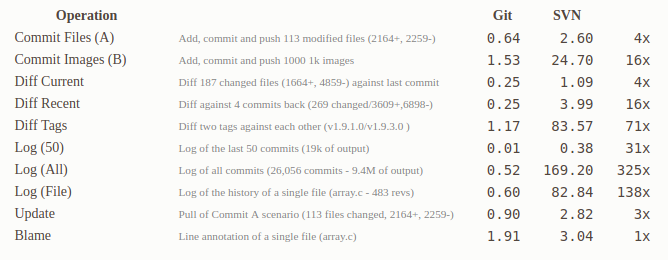
\includegraphics[scale=0.45]{images/better-git}
	\caption{Comparison of Git and SVN speeds\cite{better}}
\end{figure}

\end{frame}

\begin{frame}[allowframebreaks]{Branching}{Git vs SVN}
\subsection{Branching}
\begin{figure}
	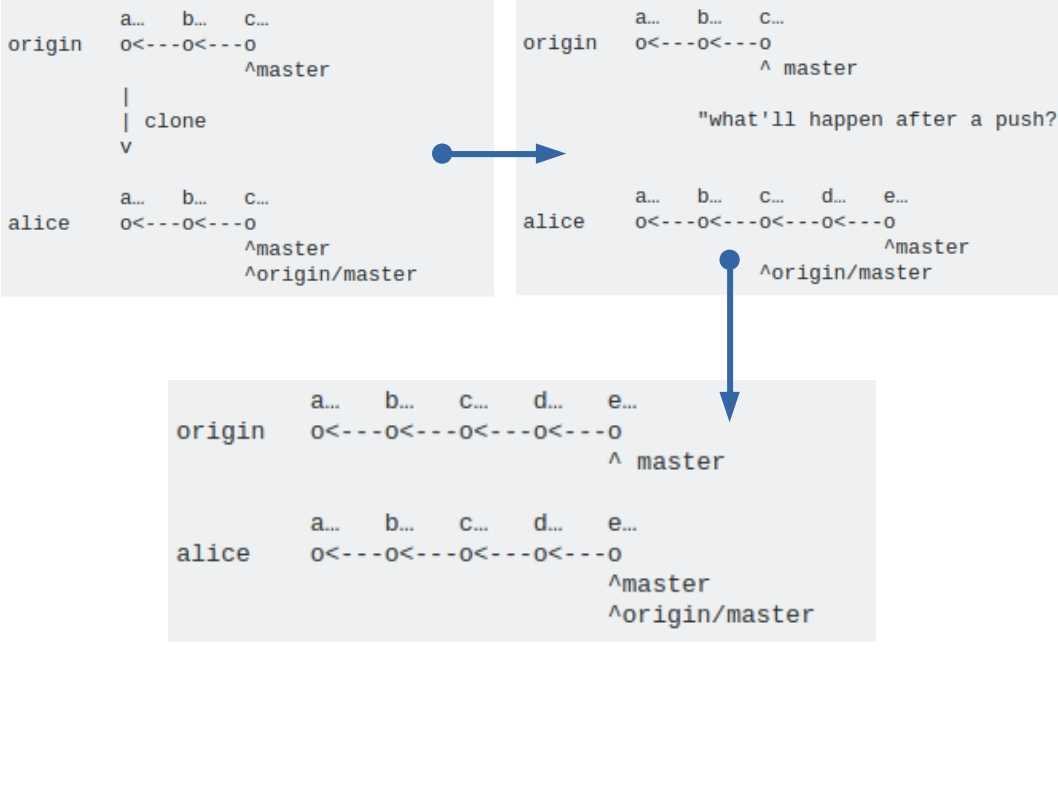
\includegraphics[scale=0.3]{images/git_vs_svn}
	\caption{Branching in Git\cite{branching}}
\end{figure}

\begin{figure}
	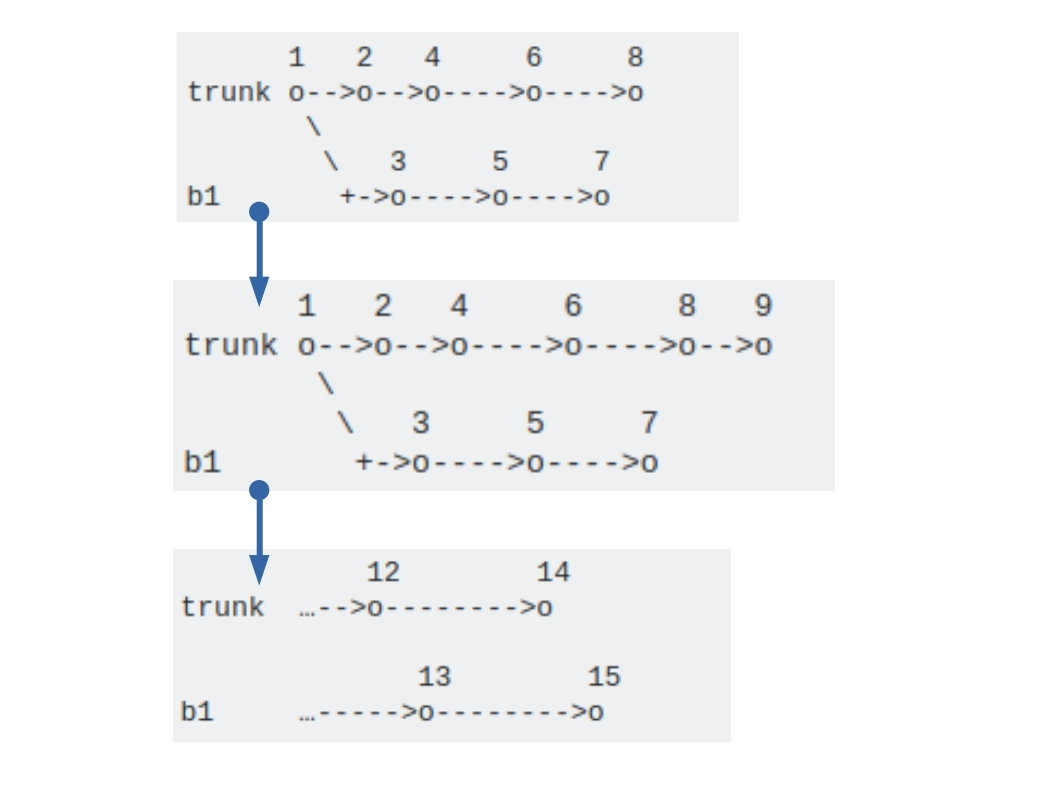
\includegraphics[scale=0.34]{images/svn.jpg}
	\caption{Branching in SVN\cite{branching}}
\end{figure}

\end{frame}



\begin{frame}{Take home message}
\section{Take home message}
\begin{itemize}
    \item There is not much difference between the most popular VCSs. It ultimately comes down to the use case.
    \item If there is a need for "Offline Source Control" with really good branching features, Git's fantastic. Open source projects are worked on with the help of Git. 
    \item If there is a need to have a strictly centralized Source Control that is simple and has excellent tooling (at least on Windows), choose SVN.
\end{itemize}
    
\end{frame}

\begin{frame}{References}
  \section{References}
    
  \begin{thebibliography}{10}


  \bibitem{naming-conv}
	\href{https://doctorfreelance.com/file-naming-conventions/}{Naming Conventions}

  \bibitem{website}
	\href{https://www.appfusions.com/display/StashSCMImporter/CVCS+vs.+DVCS+In+a+Nutshell
}{CVCS and DVCS}

  \bibitem{better}
\href{https://git-scm.com/about/small-and-fast}{Comparison between Git and SVN speeds}
	
	  \bibitem{branching}
	\href{https://stackoverflow.com/questions/2471606/how-and-or-why-is-merging-in-git-better-than-in-svn
	}{Branching SVN vs Git}
	



  \end{thebibliography}
\end{frame}

\end{document}


